% Author: Clint P. George 
% Last edited on: November 12, 2015 
% Compiles on: XeLatex and PDFLatex 

\documentclass[compress,mathserif,t]{beamer} % " mathserif " option for math, t for v-align top 
\setbeamertemplate{navigation symbols}{} % gets rid of navigation symbols
\setbeamerfont{page number in head/foot}{size=\tiny}
%\setbeamertemplate{footline}[frame number]
\setbeamertemplate{footline}{\hfill\fboxsep=1mm\fboxrule=0pt\fbox{\insertframenumber}}
%\setbeameroption{show notes}
\setbeamersize{text margin left=7mm}

%\usepackage{amsfonts}
%\usepackage{amstext}
\usepackage{amsmath}
%\usepackage{versions}
\usepackage{graphicx}
%\usepackage{times}
%\usepackage{fancyvrb}
%\usepackage{cancel}
%\usepackage{pstricks}
%\usepackage{amsthm}
\usepackage{bm}
\usepackage{subfigure}
\usepackage{accents}
\usepackage{url}
\usepackage{multirow}
\usepackage{multicol}
\useinnertheme{circles}

%%%%%%%%%%%%%%%%%%%%% RESETS THE FIGURE NUMBER %%%%%%%%%%%%%%%%%%%%%
\makeatletter
\@addtoreset{subfigure}{framenumber}
\makeatother
%%%%%%%%%%%%%%%%%%%%% RESETS THE FIGURE NUMBER %%%%%%%%%%%%%%%%%%%%%

\DeclareMathOperator{\supp}{supp}
\DeclareMathOperator*{\argmax}{argmax}
\DeclareMathOperator{\Dir}{Dir}
\DeclareMathOperator{\Mult}{Mult}

\newcommand{\commentt}[1]{}
\newcommand{\bz}{{\bm z}}
\newcommand{\bw}{{\bm w}}
\newcommand{\balpha}{\bm \alpha}
\newcommand{\bbeta}{\bm \beta}
\newcommand{\btheta}{\bm \theta}
\newcommand{\bpsi}{\bm \psi}

\newcommand{\Real}{\mathbb{R}}
\newcommand{\simplex}{\mathbb{S}}
\newcommand{\given}{\,|\,}
\newcommand{\cas}{\stackrel{\text{a.s.}}{\rightarrow}}
\newcommand{\iid}{\stackrel{\text{iid}}{\sim}}
\newcommand{\ind}{\stackrel{\text{ind}}{\sim}}
\newlength{\dhatheight}
\newcommand{\doublehat}[1]{%
    \settoheight{\dhatheight}{\ensuremath{\hat{#1}}}%
    \addtolength{\dhatheight}{-0.25ex}%
    \hat{\vphantom{\rule{1pt}{\dhatheight}}%
    \smash{\hat{#1}}}}

\newcommand{\doublehatsubscript}[1]{%
    \settoheight{\dhatheight}{\ensuremath{\hat{#1}}}%
    \addtolength{\dhatheight}{-.65ex}%
    \hat{\vphantom{\rule{1pt}{\dhatheight}}%
    \smash{\hat{#1}}}}

\title{Exploratory Data Analysis}
\author{Clint P. George}
\institute[UFII]{ University of Florida Informatics Institute\\ 
\vspace{10mm}
}
\date{\small{December $05$, $2016$}}
%\date{\today}
\begin{document}
\maketitle



\begin{frame}

\color{blue}\rule{\linewidth}{4pt}
Outline
\begin{enumerate}
	\item Principal Component Analysis (PCA)
	\item Introduction to Document Modeling 
	\item Term-Frequency Inverse Document Frequency (TF-IDF)
	\item Latent Semantic Analysis (LSA)
\end{enumerate}




\end{frame}


\section{Principle Component Analysis}


\begin{frame}
\frametitle{Principle Component Analysis: Goal}

We wish to summarize datasets which may contain several redundant 
features (or characteristics). 

\only<2>{
	
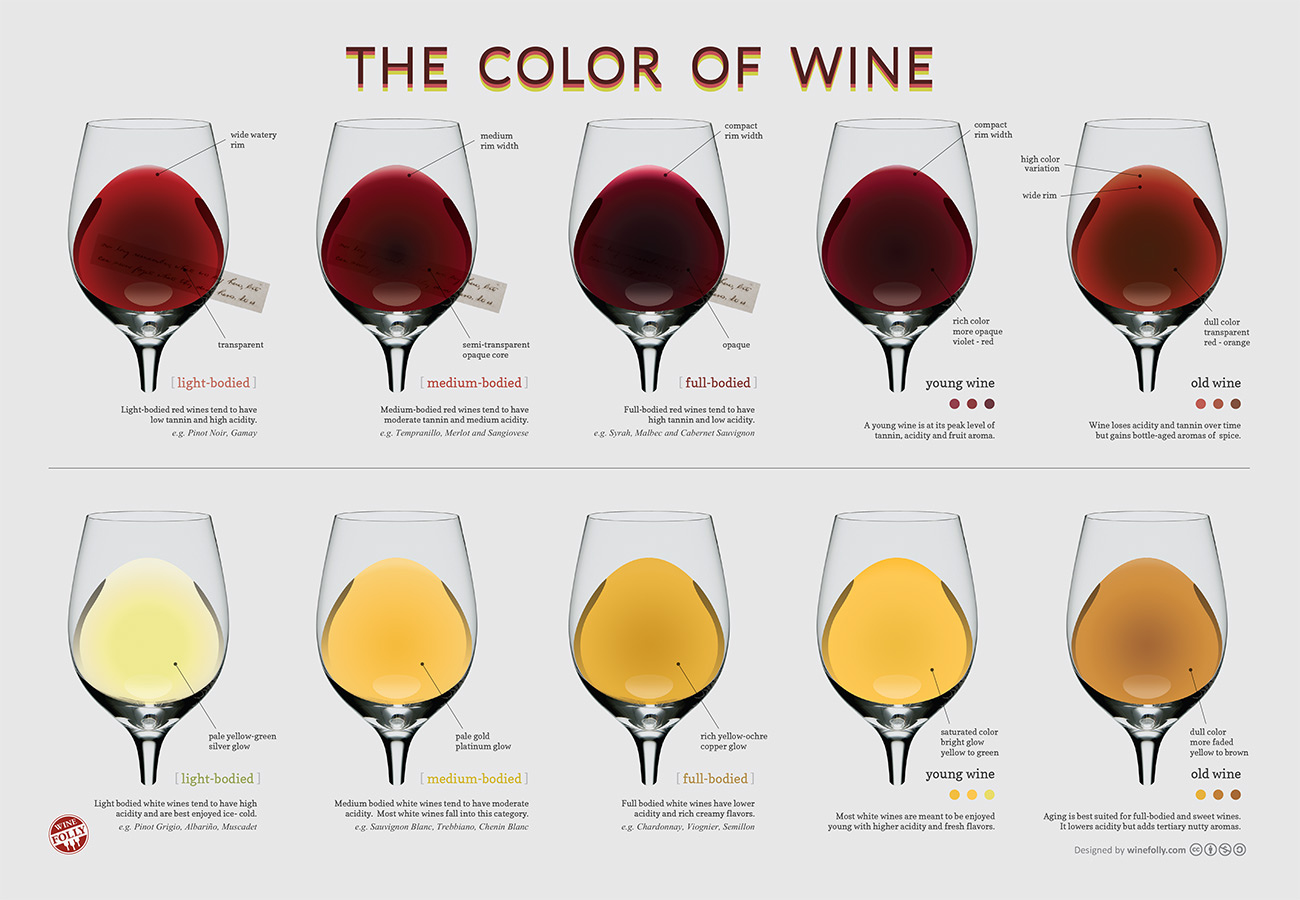
\includegraphics[width=.8\textwidth]{wine-color}

}
\only<3->{

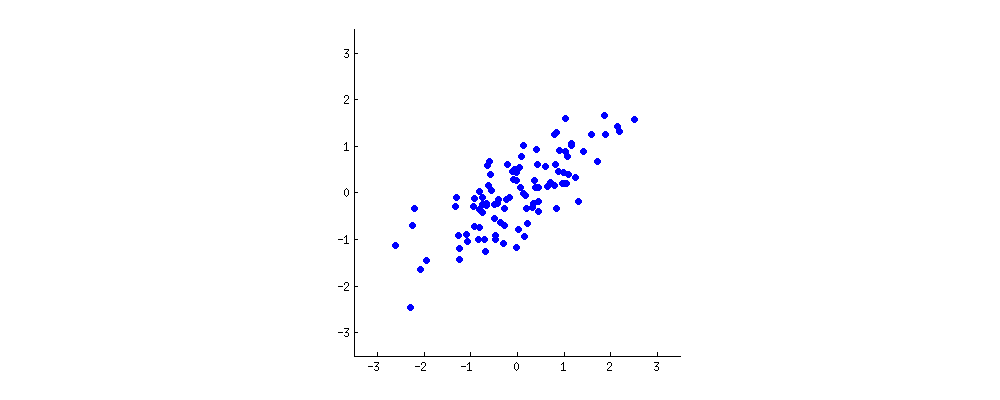
\includegraphics[width=1.1\textwidth]{jPw90}

synthetic data: $x$-axis - color intensity, $y$-axis - alcohol 
content  

}
\only<4->{
\begin{itemize}
	\item look for some features that strongly 
	differ across data points.
	\item look for the properties that would allow you to 
	``reconstruct'' well the original features		
\end{itemize}
}

	
\end{frame}

\begin{frame}{Eigenvectors and Eigenvalues: Overview}

Let $C$ be an $n \times n$ matrix and 
$\mathbf{u}$ is an $n \times 1$ vector.---
$C\mathbf{u}$ is well-defined. 

\vspace{.3cm}
Typically, multiplication by a matrix changes 
the direction of a \emph{non-zero} vector 
$\mathbf{u}$\only<2>{
\begin{columns}
\begin{column}{0.4\textwidth}
$(x_1, y_1) = (0, 0)$ 
$(x_2, y_2) = (2, 2)$
\[ 
C = \begin{bmatrix}
\cos(\frac{\pi}{4}) & \sin(\frac{\pi}{4}) \\ 
-\sin(\frac{\pi}{4}) & \cos(\frac{\pi}{4}) \\
\end{bmatrix}
\] 
\end{column}
\begin{column}{0.6\textwidth}\centering
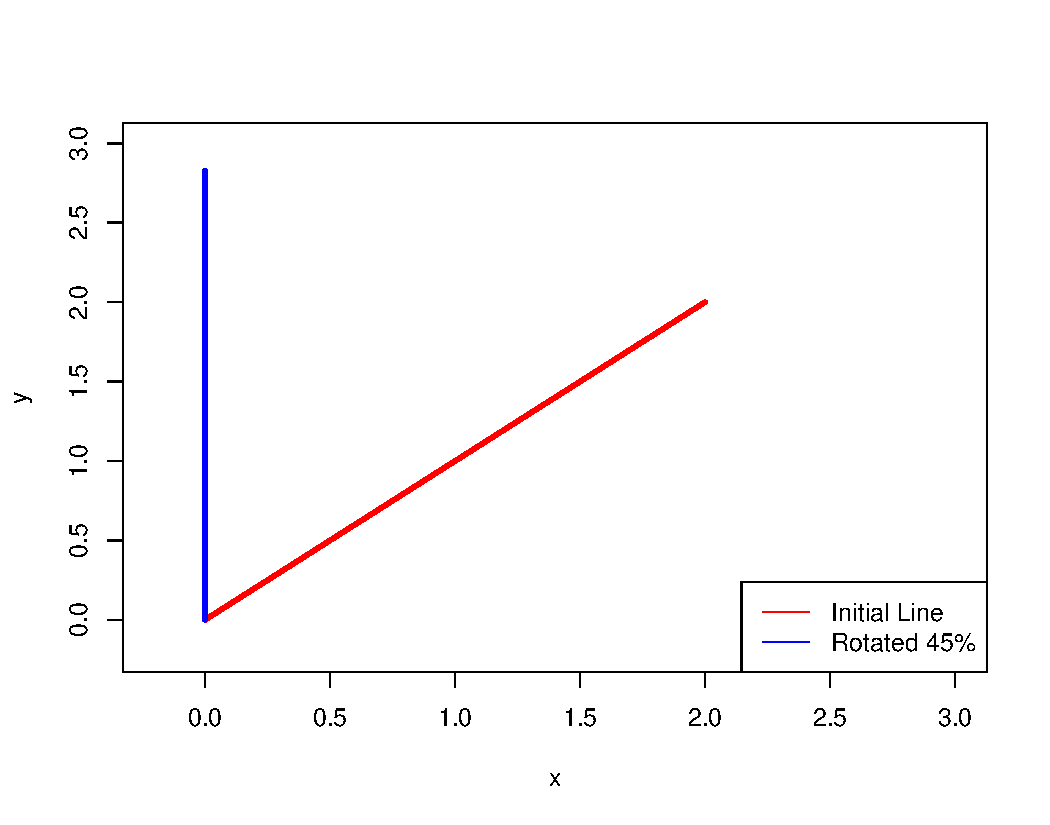
\includegraphics[width=.8\textwidth]{rotate-line}
\end{column}
\end{columns}
}\only<3->{, unless the vector is 
\emph{special} as in this transform 
$C\mathbf{u} = \lambda \mathbf{u}$, 
where $\lambda$ is a scale that $C$ performs over the 
vector $\mathbf{u}$.
} 
\only<3>{
\begin{columns}
	\begin{column}{0.4\textwidth}
%		$(x_1, y_1) = (0, 0)$ 
%		$(x_2, y_2) = (2, 2)$
		\[ 
		C = \begin{bmatrix}
		.5 & .0 \\ 
		.0 & .5 \\
		\end{bmatrix}
		\] 
	\end{column}
	\begin{column}{0.6\textwidth}\centering
		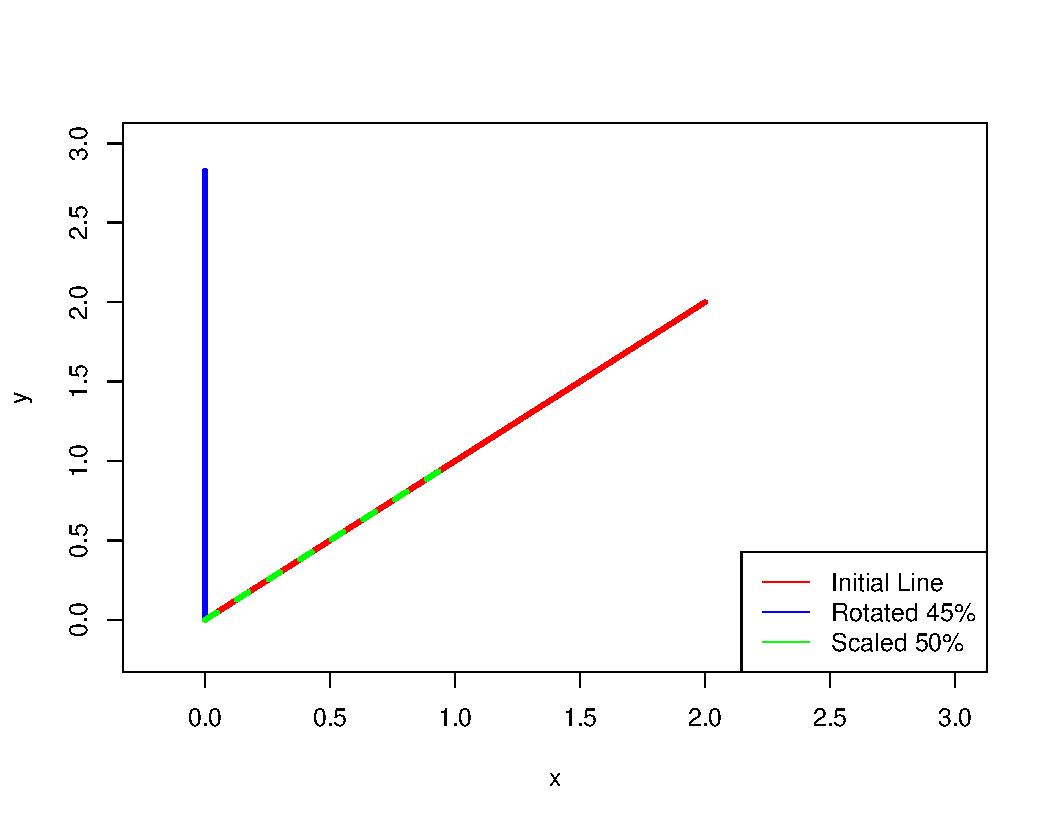
\includegraphics[width=.8\textwidth]{rotate-scale-line}
	\end{column}
\end{columns}

} 



\only<4->{
	
	\vspace{.5cm}
	
	These special vectors and their corresponding  
	$\lambda$'s are called 
	\textbf{eigenvectors} and \textbf{eigenvalues} 
	of $C$. } \only<5->{$C$ can 
	have upto $n$ distinct 
	eigenvalues. 
}

\end{frame}

\begin{frame}{Eigenvectors and Eigenvalues: Facts}
	
	Let $U$ be an $n \times n$ 
	matrix with $n$ 
	eigenvectors of $C$ and $\Lambda$ is the $n 
	\times n$ diagonal matrix with the eigenvalues 
	of $C$ along its diagonal. 
	
	\vspace{.5cm}
	
	The column vectors of $U$ are 
	linearly independent, which 
	gives 
	
	\[ C U = U \Lambda \rightarrow 
	C = 
	U \Lambda U^{-1}. \]   
	
	This \textbf{diagonalizes} 
	the matrix $C$. 
	
	\vspace{.5cm}
	
	If $C$ is symmetric ($C = C^{\text{T}}$), then 
	its eigenvectors are perpendicular and we can 
	have $U^{-1} = U^{\text{T}}$ 
	and \[ C = U \Lambda 
	U^{\text{T}} \]   
	
\end{frame}


\begin{frame}
	\frametitle{Principle Component Analysis: Approach}
	
	Let $X$ be a centered $m \times n$ data matrix.  
	% centered - column means have been 
	%subtracted and are now equal to 
	%zero.
	
	\vspace{.4cm}
	We can write the $n \times n$ 
	covariance matrix $C$ as:
	\[ C = \frac{X^\text{T} X}{n - 1} = 
	U \Lambda U^\text{T}, \] 
	where $U$ is the matrix of 
	eigenvectors $\mathbf{u}_i$ 
	(each 
	column is an 
	eigenvector) and $\Lambda$ 
	is the diagonal matrix with eigenvalues 
	$\lambda_i$ on the diagonal. 
	
	\vspace{.4cm} \only<2->{
		PCA transformation: projections of the data $X$ on the 
		\textbf{principal components}, i.e. $XU$. One only needs 
		to keep the most informative principal components. 		
	}
	
\end{frame}





\begin{frame}{Text Corpus Exploration}
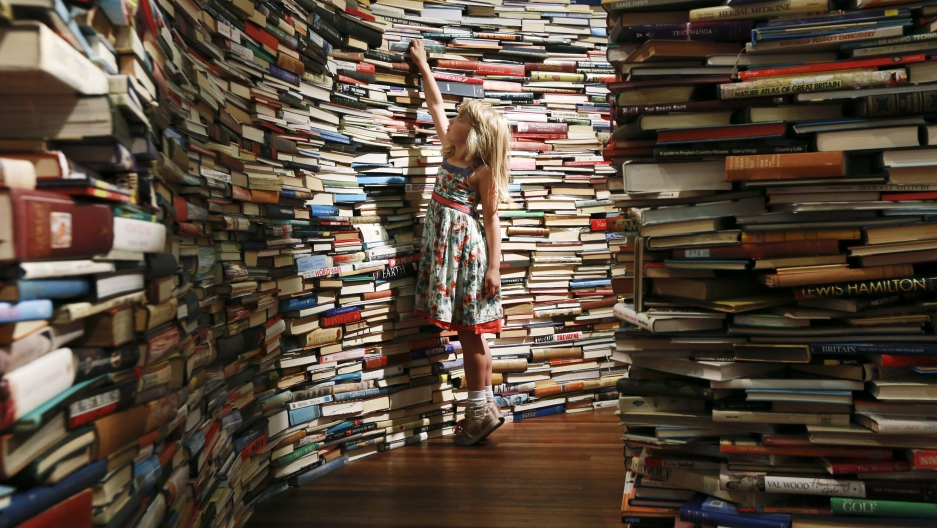
\includegraphics[width=.8\textwidth]{books-olivia-harris-reuters}

\vspace{1cm}

We have a big pile of text documents 
(corpus).---What's 
going on inside?\footnote{PC: Olivia Harris,  
Reuters} 
\end{frame}

\begin{frame}{Text Corpus Exploration}
	
\begin{itemize}
	\item Comparing document covariates---How 
	do individual words correlate?
	
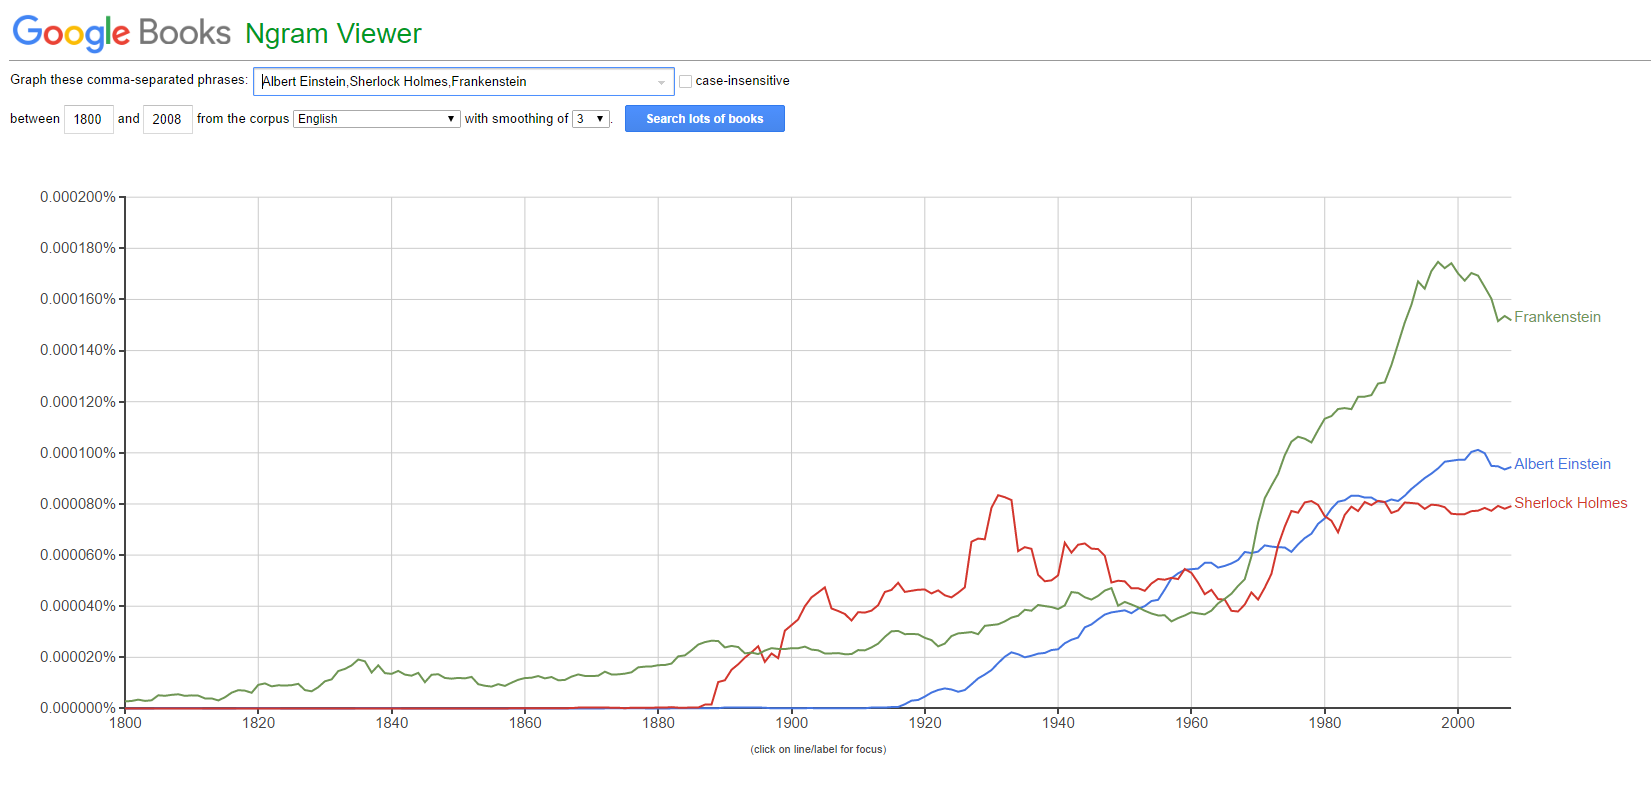
\includegraphics[width=.98\textwidth]{word-covariate-analysis}

	\item Clustering and topic modeling 
	\item Organizing and searching 
	documents---information retrieval   
\end{itemize}

\end{frame}





\section{Keyword-based Search}

\begin{frame}
	\frametitle{An Information Retrieval 
		Problem }
	
	Keyword-based search: \\[.3cm]   
	% \only<2->{
		\begin{itemize}
			\item searching for documents of 
			interest 
			\item e.g., keywords: computers, 
			laptop, etc.  
		\end{itemize}
	% }
	
	%	\only<3->{
	%		\vspace{1cm}
	%		How do we do it?
	%	}
	
\end{frame}

\begin{frame}
	\frametitle{Implementing Keyword-based 
	Search} 
	
	An approach is via \textbf{Vector Space 
	Modeling}
	\begin{itemize}
		\item Convert a corpus $m$ 
		documents 
		and $n$ vocabulary terms 
		into a 
		\textbf{term-document} ($n 
		\times m$) 
		matrix
		% each cell represents a term's 
		%relative frequency
		% column represents a document 
		
		\item Translate both 
		\textcolor{blue}{documents} and 
		\textcolor{blue}{user keywords} 
		into vectors in vector space
		
		\item Define similarity between these 
		vectors, e.g., via cosine 
		similarity---small angle $\equiv$ 
		large cosine $\equiv$ similar 
		
	\end{itemize}
	
\end{frame}

\begin{frame}{TF-IDF} 
	
	Term frequency inverse document frequency 
	matrix (TF-IDF)\footnote{Salton et al. 
	(1975)}---a popular scheme
	
	\vspace{1cm}
	
	For each term $t$ in document $d$, we 
	compute 
	\[ \text{tf-idf}_{dt}  = \text{tf}_{dt} 
	\times \log  \left ( 
	\frac{n}{\text{df}_{t}} \right )  \]
	\begin{itemize}
		\item $\text{tf}_{dt}$ is the 
		frequency of term $t$ in document $d$
		\item $\text{df}_{t}$ is the number of 
		documents where term $t$ 
		appears
	\end{itemize}
	
	
\end{frame}


\begin{frame}[plain,c]
	
	\begin{center}
		
		Hands-on Python: TF-IDF and 
		document retrieval 
		
	\end{center}
	
\end{frame}

\begin{frame}
	\frametitle{Information Retrieval: Challenges}
	
	If we search for the keyword 
	\textcolor{blue}{\emph{computers}}, we 
	may miss documents that do not have 
	\emph{computers} and contain 
	\textcolor{blue}{\emph{PC}}, 
	\textcolor{blue}{\emph{laptop}}, 
	\textcolor{blue}{\emph{desktop}}, etc. 
	\\[.3cm]   
	\only<2->{
		\begin{itemize}
			\item \textcolor{red}{Problem \#1: 
				Synonymy}---words with similar 
			meaning %, e.g., \emph{car} and 
			%\emph{automobile}
		\end{itemize}
	}
	
	\only<3->{
		\vspace{.5cm}
		Suppose, we search for the keyword 
		\textcolor{blue}{\emph{chair}}, we 
		may get documents that contain ``the 
		\textcolor{blue}{chair} of 
		the board'' and ``the 
		\textcolor{blue}{chair} maker''\\[.3cm]
	}\only<4->{
		\begin{itemize}
			\item \textcolor{red}{Problem \#2: 
				Polysemy}---words with multiple 
			meanings
		\end{itemize}
	}
	
	
	\only<5->{
		\vspace{1.5cm}
		
		One solution: search and explore 
		documents based on the themes or 
		\textbf{topics} that run through them. 
		
		\note{
			\begin{itemize}
				\item Synonymy leads to poor 
				\emph{Recall} (the fraction of 
				all 
				relevant documents that are 
				retrieved)
				\item Polysemy leads to many 
				false positives (low 
				\emph{Precision})
			\end{itemize}
		}
	}
\end{frame}


\begin{frame}[noframenumbering]{TF-IDF} 
	
	Term frequency inverse document frequency matrix 
	(TF-IDF)\footnote{Salton et al. (1975)}---a popular scheme
	
	\vspace{1cm}
	
	For each term $t$ in document $d$, we 
	compute 
	\[ \text{tf-idf}_{dt}  = \text{tf}_{dt} 
	\times \log  \left ( 
	\frac{n}{\text{df}_{t}} \right )  \]
	\begin{itemize}
		\item $\text{tf}_{dt}$ is the 
		frequency of term $t$ in document $d$
		\item $\text{df}_{t}$ is the number of 
		documents where term $t$ 
		appears
	\end{itemize}
	
	\vspace{1cm}
	
	\textcolor{red}{Problem \#3: Working 
		in the vocabulary space can cause 
		computational challenges for large 
		corpora.}
	
\end{frame}

\begin{frame}
	\frametitle{The Curse of Dimensionality\footnote{Bellman (1961)}}
	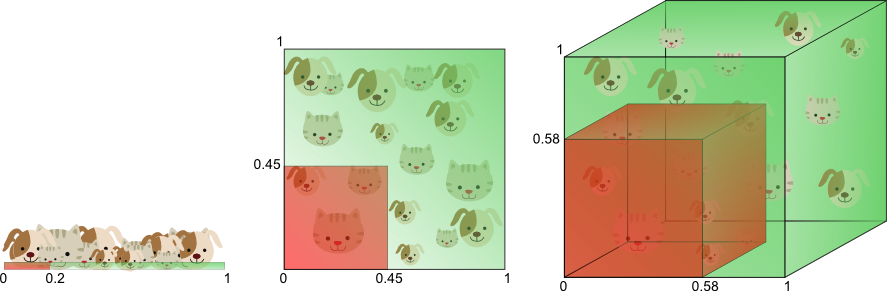
\includegraphics[width=1.\linewidth]{curseofdimensionality}
	
	%definition: the impossibility of 
	%optimizing a function of many 
	%variables by a brute force search on a 
	%discrete multidimensional 
	%grid. (The number of grid points 
	%increases exponentially with 
	%dimensionality)
	
	Suppose the available data (documents) are 
	fixed and we keep adding 
	dimensions (words).\footnote{Image source: 
		\url{www.visiondummy.com}} 
	\\  
	\vspace{1cm}
	
	The more features we use, the more sparse 
	the data becomes
	
	%Another effect of the curse of 
	%dimensionality, is that this 
	%sparseness is not uniformly distributed 
	%over the search space. In 
	%fact, data around the origin (at the 
	%center of the hypercube) is 
	%much more sparse than data in the corners 
	%of the search space. 
	
	%widely observed phenomenon that data 
	%analysis techniques (including
	%clustering), which work well at lower 
	%dimensions, often perform 
	%poorly as the dimensionality of the 
	%analyzed data increases. 
	
\end{frame}








\section{Latent Semantic Analysis}


\begin{frame}{Latent Semantic Analysis (LSA)}

LSA (Deerwester et al. 1990) aims to explore  
the ``semantics'' underlying documents.   

\vspace{1cm}
By factorizing the TF-IDF ($n 
\times m$) 
matrix---Singular Value Decomposition

\end{frame}



\begin{frame}{Singular Value Decomposition 	
(SVD)}

Let $A$ be an $m \times n$ matrix with real 
values and $m > n$. Let $B = A^{\text{T}} A$ 
be an $n \times n$ matrix.---it's symmetric.

\only<2->{
	\vspace{.4cm}
	
	The eigenvalues, $\sigma_1, \ldots, \sigma_n$, 
	of such matrices are real non-negative numbers. 
	We then can write: $\sigma^2_1 \geq 
	\sigma^2_2 \geq \ldots \geq  \sigma^2_n$. 
%	Typically, for some index $r \leq n$, the first $r$ 
%	numbers $\sigma_1, \ldots, \sigma_r$  are 
%	positive whereas the rest are zero. 
}

\only<3->{
\vspace{.4cm}

The corresponding eigenvectors $\mathbf{u}_1, 
\ldots, \mathbf{u}_n$ are perpendicular. 
We normalize them to have length $1$. Let 
\[ U = [\mathbf{u}_1, \ldots, 
\mathbf{u}_n] 
\text{ and } 
 V = [\mathbf{v}_1, \ldots, 
 \mathbf{v}_n] 
\] 
where we define $\mathbf{v}_i = 
\frac{1}{\sigma_i} A 
\mathbf{u}_i$. 
}

\only<4->{
\vspace{.4cm}

\textcolor{blue}{
We can easily show that 
$\mathbf{v}_i$'s are perpendicular 
$m$-dimensional vectors of length $1$ 
(orthonormal vectors).}
}
\end{frame}

\begin{frame}{Singular Value Decomposition (SVD)}
	
By construction, we have 
\[ \mathbf{v}^{\text{T}}_j A 
\mathbf{u}_i 
= \mathbf{v}^{\text{T}}_j 
(\sigma_i 
\mathbf{v}_i) 
= \sigma_i 
\mathbf{v}^{\text{T}}_j 
\mathbf{v}_i 
= \begin{cases}
\sigma_i,& \text{if } i = j\\
0,              & \text{otherwise} 
\end{cases}
\] 

\only<2->{
\vspace{.4cm}

We can then write the matrix form: 

\[ V^{\text{T}} A U = \Sigma \]
where $\Sigma$ is the diagonal $n \times n$ 
matrix with $\sigma_1, \ldots, \sigma_n$ along 
the diagonal.---singular values. 
}

\only<3->{
\vspace{.4cm}

Since $U$ and $V$ have orthonormal 
columns, we can have $A  = V 
\Sigma U^{\text{T}}$
}
	
\end{frame}


\begin{frame}
\frametitle{Singular Value Decomposition 
	(SVD): Summary}

SVD factorizes an $m \times n$ data matrix 
$A$ into: 
%the product of an 
%orthogonal matrix $U$, a diagonal matrix 
%$S$, and the transpose of 
%an orthogonal matrix $V$:
\[ A_{m \times n} = V_{m \times n} 
\: 
\Sigma_{n \times n} \: U_{n \times 
	n}^\text{T} \]
\only<2->{where the columns of 
$U$ are eigenvectors  of 
$A^\text{T}A$}
%\only<3->{% the columns of V are 
%	% eigenvectors of $AA^\text{T}$,  
%$U^\text{T}U = I$ and $V^\text{T}V = I$, % 
%%orthonormal
%}
\only<3->{and $\Sigma$ is a diagonal matrix 
	containing the square roots of eigenvalues 
	of $A^\text{T}A$ in descending order.}

\vspace{.5cm}

\only<5->{
In LSA, we set all but the $(K \ll n)$ 
highest singular 
values to 
$0$, giving a $K \times n$ 
approximation matrix---the 
``semantic'' 
space
}

\only<6->{
\vspace{.3cm}
One can identify \textbf{similarities} 
between documents in this 
\textbf{semantic space}. 
}

%Remember that the number of non-zero singular 
%values equals the rank of the matrix. 
	
\end{frame}


\begin{frame}{SVD: Geometric Interpretation}

\begin{multicols}{2} 
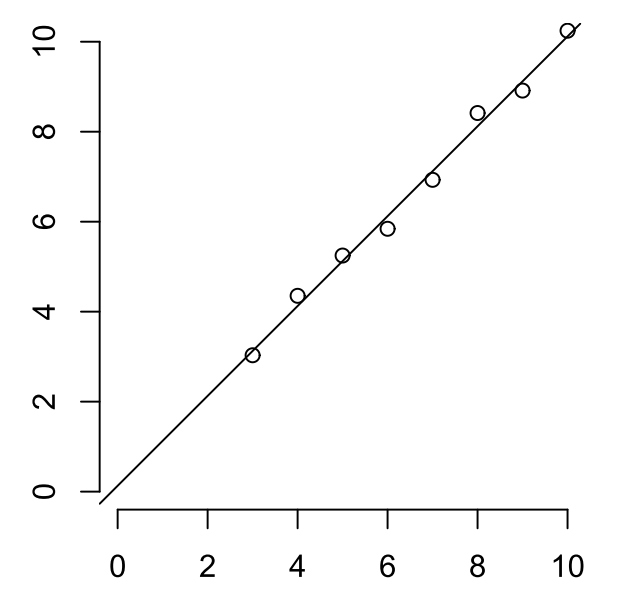
\includegraphics[width=.45\textwidth]{svd-eg-01}
\\ \vspace{-2mm}
\small{Regression line along $1$st 
dimension} \vspace{-2mm}
\columnbreak \\
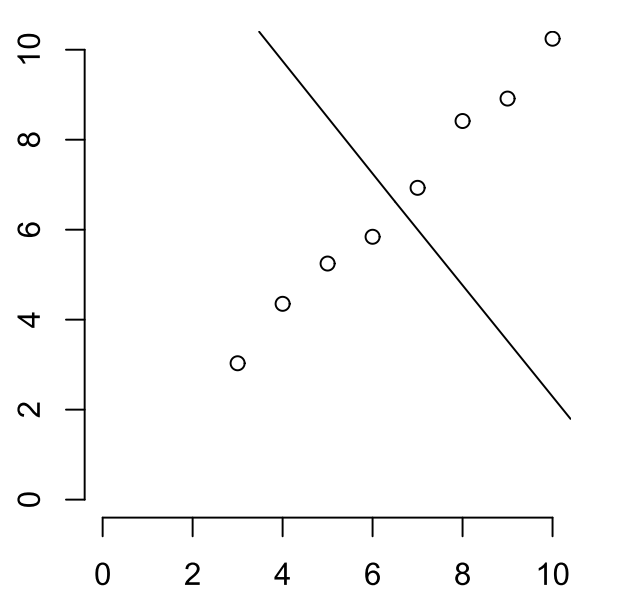
\includegraphics[width=.45\textwidth]{svd-eg-02}
\\ \vspace{-2mm}
\small{Regression line along $2$nd 
dimension} \vspace{-2mm}
\end{multicols}

%We use these regression lines to generate 
%a set of uncorrelated data 
%points that will show sub groupings in 
%the original data not 
%necessarily visible at first glance.

%taking a high dimensional, highly 
%variable set of data points and 
%reducing it to a lower dimensional space 
%that exposes the 
%substructure of the original data more 
%clearly and orders it from 
%most variation to the least.

\only<2>{
The regression line on the $1$st 
dimension (left) is the best 
approximation for 
the data---it is the line that 
minimizes the distance between each 
point 
and the line.
}
\only<3>{
The regression line on the $2$nd 
dimension (right) does a poorer job of 
approximating the data, because it 
corresponds to a dimension exhibiting 
less 
variation
}
\only<4->{
SVD aims to find the dimensions along 
which data points 
exhibit the most variation.
}

%The SVD is what you get when you iteratively solve the greedy 
%optimization problem of fitting data to a line.

% We can see it as a method for 
%transforming correlated variables into a 
%set of 
% uncorrelated ones that better expose the 
%various relationships among the 
% original data items. 
% SVD is a method for identifying and 
%ordering the dimensions along which data 
% points exhibit the most variation. This 
%ties in to the third way of viewing 
% SVD, which is that once we have 
%identified where the most variation is, 
%it’s 
% possible to find the best approximation 
%of the original data points using 
% fewer dimensions. Hence, SVD can be seen 
%as a method for data reduction.

\end{frame}


\begin{frame}{Application of SVD: Data Compression}
	
	\begin{multicols}{2} 
		
\includegraphics[width=.29\textwidth]{svd-O}
		\\ \vspace{-2mm}
		\small{$25 \times 15$ gray-scale 
		image ($375$ cells)} \vspace{-2mm}
		\columnbreak \\
		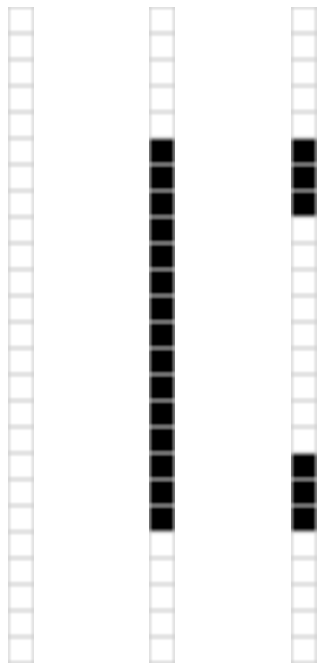
\includegraphics[width=.24\textwidth]{svd-O-features}
		\\ \vspace{-2mm}
		\small{Three types of 
		columns/features} 
		\vspace{-2mm}
	\end{multicols}
	SVD on the matrix, $A$, gives three 
	non-zero singular values.\footnote{		
	Example from: 
	http://www.ams.org/samplings/feature-column/fcarc-svd}
		    
\end{frame}

\begin{frame}[plain,c]
	
	\begin{center}
		
		Hands-on Python: Latent Semantic 
		Analysis 
		
	\end{center}
	
\end{frame}

\begin{frame}
\frametitle{PCA vs LSA}
We assume a \textsl{centered} data matrix $X$. We write its  
covariance matrix $C$  
as\footnote{\url{http://stats.stackexchange.com/questions/134282}}
 
\begin{eqnarray}
C &=& \frac{X^\text{T} X}{n - 1} \\ 
  &=& \frac{USV^\text{T} 
  VSU^\text{T}}{n - 1} 
\text{ (using SVD) } \\ 
	&=& U\frac{S^2}{n - 
	1}U^\text{T}
\label{eq:}
\end{eqnarray}
\only<2->{

Note: The right singular vectors 
$U$ are 
principal axes, and 
singular values are related to the 
eigenvalues of the covariance 
matrix $C$ via $\lambda_i = s_i^2 /(n - 1)$. 
}

\end{frame}

\begin{frame}[plain,c]
	
	\begin{center}
		
		\Huge Questions? 
		
	\end{center}
	
\end{frame}


%\begin{frame}
%\frametitle{Dataset for Comparison}
%
%A corpus created from a subset of Wikipedia 
%articles
%\begin{table}[ht]
%  \begin{tabular}{p{5cm} r} \hline
%    Categories & Vocabulary size \\ \hline 
%		Eagles ($62$) & $2{,}113$ \\ 
%		Owls ($76$)   & \\ \hline	
%  \end{tabular}
%\end{table}
%
%We removed stop words and words with 
%frequency less than $10$ in the 
%corpus. 
% 
%\end{frame}
%
%\begin{frame}
%\frametitle{LSA: Analysis of Results}
%
%
%\begin{multicols}{2} \centering 
%\textbf{Component-1} \\
%\small{
%alike(-0.00067), savannah(-0.0013), 
%peter(-0.002), 
%disputed(-0.0021), nepal(-0.0022), 
%javan(-0.0022), 
%scops-owl(-0.0023), bangladesh(-0.0024), 
%behavioral(-0.0024), 
%cirrhatus(-0.0025), cuba(-0.0025), 
%subtropical(-0.0026), 
%asl(-0.0027), junior(-0.0028), 
%peninsular(-0.0028), 
%nowadays(-0.0028), correct(-0.0029), 
%earless(-0.003), page(-0.003)}
%\columnbreak 
%
%\textbf{Component-2} \\ 
%\small{ verreaux(0.095),     
%eagle(0.088),        
%crowned(0.088),      harpy(0.084),       
%hyrax(0.074),       martial(0.074),      
%lamb(0.073),         
%monkey(0.071),      
%booted(0.071),       home(0.068),         
%golden(0.068),       
%fledging(0.067),    
%wedge-tailed(0.066), national(0.066),     
%ethiopia(0.064),     
%aquila(0.064),      
%carrion(0.058),      sheep(0.055),        
%kg(0.054)    
%}
%\end{multicols}
%      
%
%The number of LSA components $k = 2$.---based 
%on the left singular 
%matrix $U$.     
%
%\end{frame}
%
%
%\begin{frame}
%\frametitle{LSA: Analysis of Results}
%
%\begin{figure}[h]
%\centering
%\vspace{-.8cm}
%\includegraphics[width=.8\textwidth]{eagles-owls-lsa-space}
%\end{figure}
%
%Blue circles represent $62$ Eagle articles 
%and red circles 
%represent $76$ Owl articles.---based on the 
%right singular matrix 
%$V$.     
%
%\end{frame}
%
%
%
%
%\end{frame}
%
%\begin{frame}
%\frametitle{PCA: Analysis of Results}
%
%\begin{figure}[h]
%\centering
%\vspace{-.8cm}
%\includegraphics[width=.8\textwidth]{eagles-owls-pca-space}
%\end{figure}
%
%Blue circles represent $62$ Eagle articles 
%and red circles 
%represent $76$ Owl articles.---We show two 
%principal components.  
%
%
%
%\end{frame}
%
%
%\begin{frame}
%\frametitle{Latent Dirichlet Allocation (LDA, 
%Blei et al. '03)}
%
%\begin{figure}[h]\vspace{-1cm}
%\centering
%\includegraphics[width=1.08\textwidth]{lda-intuition}
%\end{figure}
%
%LDA is a probabilistic, generative model for 
%a corpus\footnote{This 
%example is 
%taken from Blei (2012)}. 
%\note{
%This model can be best explained by its 
%generative random process.
%
%\begin{itemize}
%	\item A topic is a distribution over the 
%vocabulary. For example, 
%	the topic \emph{Sports} has words such as 
%\emph{football}, 
%	\emph{soccer}, \emph{etc.}, with high 
%probability.   
%	\item Each document is assumed to be 
%generated as follows. First 
%	choose a distribution over the topics (the 
%histogram at right); 
%	then, for each word, choose a topic 
%assignment (the colored 
%coins) 
%	and choose the word from the corresponding 
%topic. 
%\end{itemize}
%
%Topic modeling enables us to organize and 
%summarize electronic
%archives at a scale that would be impossible 
%by human annotation.\\ 
%\vspace{.5cm}
%
%We would like to make inference on the latent 
%topic variables for 
%the corpus and cluster together documents 
%which are similar. 
%}
%
%
%\end{frame}
%
%
%\begin{frame}
%\frametitle{LDA: The Hierarchical Model}
%
%Notation and Terminology
%
%\begin{itemize} % [<+->]
%
%\item We have a vocabulary ${\cal V}$ of $V$ 
%words in the corpus, 
%and 
%
%\item $D$ documents in the corpus, and for $d 
%= 1, \ldots, D$, 
%document $d$ has $n_d$ words, $w_{d1}, 
%\ldots, w_{dn_d}$
%
%\item A topic is a distribution over ${\cal 
%V}$. The \textbf{number 
%of topics $K$} is known. 
%
%\item Let $h = (\eta, \alpha) \in (0, 
%\infty)^{2}$ be the 
%\textbf{hyperparameter} vector 
%
%\end{itemize}
%
%\end{frame}
%
%
%\begin{frame}[noframenumbering]
%\frametitle{LDA: The Hierarchical Model}
%
%\begin{figure}[htbp]
%\centering
%\includegraphics[width=.85\textwidth]{lda-hierarchical-model}
%\end{figure}
%
%
%The Hierarchical Model 
%
%\begin{enumerate} % [<+->]
%
%\item $\beta_t \iid \Dir_V(\eta, \ldots, 
%\eta)$, for $t = 1, \ldots, 
%K$.
%
%\item $\theta_d \iid \Dir_K(\alpha, \ldots, 
%\alpha)$, for $d = 1, 
%\ldots, D$. 
%
%\item Given $\theta_d$, $z_{di} \iid 
%\Mult_K(\theta_d)$, for $i = 1, 
%\ldots, n_d$, 
%$d = 1, \ldots, D$. 
%
%\item Given $\bbeta$ and $z_{di}$, draw 
%$w_{di}$ 
%independently from the row of $\bbeta$ 
%indicated by $z_{di}$, for $i 
%= 1, \ldots, n_d, \, d = 1, \ldots, D$.
%
%\end{enumerate}
%
%\note{
%
%
%
%\begin{itemize}
%	\item The samples $\beta_1, \beta_2, 
%\ldots, \beta_K$ form a $K 
%\times V$ matrix 
%	\item $\theta_d$'s are independent of 
%$\beta_t$'s. 
%	\item Given the $\theta$'s, the vectors 
%$(z_{11}, \ldots, 
%	z_{1n_1})$, $\ldots$, $(z_{D1}, \ldots, 
%z_{Dn_D})$ are 
%independent.
%	
%\end{itemize}
%
%
%}
%
%
%\end{frame}
%
%
%%
%%
%%\begin{frame}
%%\frametitle{LDA: Posterior Inference}
%%
%%
%%Let $\btheta = (\theta_1, \ldots, 
%%\theta_D)$, $\bbeta = 
%%(\beta_1, \ldots, \beta_K)$, $\bz_d = 
%%(z_{d1}, \ldots, z_{dn_d}), 
%%\, d = 1, \ldots, D$, and $\bz = (\bz_1, 
%%\ldots, \bz_D)$
%%
%%\vspace{.4cm}
%%
%%We are interested in the posterior 
%%distribution of $\bpsi 
%%:= (\bbeta, \btheta, \bz)$, given the 
%%observed words $\bw$
%%\begin{equation*}
%  %\nu_{h,\bw}(\bpsi) = \frac 
%%{\ell_{\bw}(\bpsi) 
%	%\nu_h(\bpsi)}{m_{\bw}(h)}
%%\end{equation*}
%%
%%
%%\note{
%%
%%\begin{itemize} 
%%
%%\item $\ell_{\bw}(\bpsi)$ denotes the 
%%likelihood function 
%%
%%\item $\nu_h(\bpsi)$ denotes the prior  
%%
%%\item $m_{\bw}(h)$ denotes the marginal 
%%likelihood of the data 
%%indexed by $h$, which plays an important 
%%role in inference 
%%
%%\item When $\eta$ is large, the topics tend 
%%to spread their mass 
%%evenly among many words in the vocabulary, 
%%whereas when $\eta$ is 
%%small, the topics tend to put most of their 
%%mass on only a few 
%%words.
%%
%%\item When $\alpha$ is large, each document 
%%tends to involve many 
%%different topics
%%
%%\end{itemize}
%%
%%}
%%
%%
%%
%%\end{frame}
%
%
%\begin{frame}
%\frametitle{LDA: Analysis of Results}
%
%
%\begin{multicols}{2} \centering 
%\textbf{Topic-1} \\
%\small{
%eagle(0.083)       specie(0.02)       nest(0.019)        
%bird(0.016)       
%prey(0.015)        golden(0.015)      large(0.0097)      
%female(0.0081)    
%range(0.0079)      adult(0.0078)      pair(0.0076)       
%wing(0.0076)      
%breeding(0.0074)   found(0.0073)      egg(0.0071)        
%lb(0.007)         
%area(0.007)        cm(0.0069)         habitat(0.0069)    
%population(0.0064)
%}
%\columnbreak 
%
%\textbf{Topic-2} \\ 
%\small{ 
%
%owl(0.1)         specie(0.025)    great(0.019)     bird(0.014)      
%prey(0.013)     
%eagle-owl(0.012) nest(0.012)      found(0.0096)    bubo(0.0081)     
%range(0.0077)   
%genus(0.0077)    eurasian(0.0076) large(0.0075)    female(0.0075)   
%wing(0.0072)    
%northern(0.007)  size(0.0067)     male(0.0066)     brown(0.0061)    
%north(0.0059) 
%  
%}
%\end{multicols}
%      
%
%The number of topics $k = 2$.   
%
%\end{frame}
%
%
%\begin{frame}
%\frametitle{LDA: Analysis of Results}
%
%\begin{figure}[h]
%\centering
%\vspace{-.8cm}
%\includegraphics[width=.8\textwidth]{eagles-owls-lda-space}
%\end{figure}
%
%Blue circles represent $62$ Eagle articles and red circles 
%represent $76$ Owl articles. 
%
%\end{frame}
%
%
%
%\begin{frame}
%\frametitle{$k$-means Algorithm}
%
%Our goal is to partition the data set $X$ (consists of $n$ 
%observations and $p$ 
%features) into some number of $k$ clusters. 
%% A cluster: a group of data points where inter-point distances are 
%% small compared to the distances to points outside of the cluster
%\vspace{.3cm}
%
%\only<2->{
%We introduce $p$-dimensional cluster centroids, $\mu_j, \: j = 1, 2, 
%\ldots, k$, 
%and binary indicator variables $\text{r}_{ij} \in \{ 0, 1 \}, \: j = 
%1, 2, 
%\ldots, k$ for each observation $i$.}\only<3->{The objective is to 
%minimize% of the $k$-means algorithm 
%
%\[ Q = \sum_{i=1}^{n} \sum_{j=1}^{k} \text{r}_{ij} {\| x_i - \mu_j 
%\|}_2 \]}
%\only<4->{via an \textbf{iterative optimization} scheme (after 
%initializing 
%$\mu_j$s) with two steps\footnote{Bishop (2006)}: 
%
%\begin{enumerate}
%	\item minimize $Q$ w.r.t. $\text{r}_{ij}$s, keeping  $\mu_j$s 
%fixed
%	\item minimize $Q$ w.r.t. $\mu_j$s, keeping $\text{r}_{ij}$s fixed
%\end{enumerate}
%}
%
%\end{frame}
%
%\begin{frame}
%\frametitle{$k$-means Algorithm: Illustration}
%
%Old Faithful data set: Old Faithful is a hydrothermal geyser in the  
%Yellowstone National Park. This data set consists of $272$ 
%observations, each 
%of which---i.e. an eruption---contains the duration of the eruption 
%and the time until next eruption. 
%
%\vspace{.3cm}
%
%\only<2>{
%\includegraphics[width=.85\textwidth]{kmeans-01}  
%
%Iteration \#1: (a) the data set in a two-dimensional space, 
%with initial choices for centers. (b) step-1: each 
%data point is assigned either to the red cluster or to the blue 
%cluster, according to which cluster center is nearer. (c) step-2: 
%each cluster center is re-computed to be the mean of the points 
%assigned to the corresponding cluster.
%}
%\only<3>{
%\includegraphics[width=.85\textwidth]{kmeans-02} 
%
%Iteration \#2: successive step-1, step-2, and step-1 
%}
%\only<4>{
%\includegraphics[width=.85\textwidth]{kmeans-03}  
%
%Iteration \#3: successive step-2, step-1, and step-2 
%}
%
%\end{frame}
%
%












\end{document}